\chapter{Create a Mesh from a Grid}
In this chapter, we show how to create a mesh with \Atlas 
starting from a grid. We assume that the reader already 
knows how to create a grid (see \chap{chap:global-grids}). 
% 
\begin{notebox}
With the term \textit{grid} we intend a list of points 
without any specific connectivity rule, while with the 
term mesh we intend a list of points with well-specified 
connectivity rules.
\end{notebox}
%
As before, we show both the C++ and Fortran version 
for this example.


\section{C++ version}
The \lista{code-meshes-C} shows how to construct a mesh 
starting from a grid.
%
\lstinputlisting[caption=Generating a mesh starting from a grid 
in \Atlas using C++, style=CStyle, label=code-meshes-C]{meshes-Structured.cc}
%
Once defined the command-line behaviour, we first create 
a global structured grid object (see line 24). For more 
details on how to create a grid see \chap{chap:global-grids}.

We then create a 
\inltc{mesh::generators::Structured} object called \inltc{generate\_mesh}
that will allow us to generate the mesh starting from
a structured grid.
We successively create a mesh object, \inltc{mesh} 
of the \inltc{Mesh} type on line 27 using the mesh generator.

In this simple example we took the freedom to add a few 
lines to show how to visualize the mesh in Gmsh. In particular, 
on line 29 we define a Gmsh object called \inltc{gmsh} that 
will be used to generate a Gmsh output. On line 30 we specify 
that we want to have some information regarding the mesh - this 
is achieved by defining as \inltc{true} the tag \inltc{"info"}.
Between line 31 and 35, we add two additional lines to visualize 
the mesh in 3D if required on the command-line.
Finally, on line 36 we write the mesh and save it into \inltc{mesh.msh}.
Note that the file containing the information on the mesh 
just created is called \inltc{mesh\_info.msh}.

It is now possible to run this simple program by using 
two command-line arguments representing the keyword that 
identifies an \Atlas predefined grid and the visualization 
type we want (either 2D or 3D), respectively. For instance, 
we can execute the following command line
%
\begin{lstlisting}[style=BashStyle]
./atlas_c-meshes-Structured
\end{lstlisting}
% 
This will produce an octahedral reduced Gaussian mesh 
(stored in mesh.msh) with 32 latitudes on one emisphere 
(i.e. 64 latitudes in total). It will also produce an 
additional file, called \inltc{mesh\_info.msh}, containing
some information regarding the mesh.
Note that we used the additional command-line argument 
\inlsh{--visualize 3D}. This will produce a 3D representation 
of the mesh, such as the one depicted in left side of 
\fig{fig:meshes}.

We can re-run the executable file in order to obtain 
a 2D representation as follows:
%
\begin{lstlisting}[style=BashStyle]
./atlas_c-meshes-Structured --grid O32 --visualize 2D
\end{lstlisting}
% 
This will produce a representation of the mesh like 
the one depicted on the right side of \fig{fig:meshes}.
%
\begin{figure}%
\centering
\subfloat{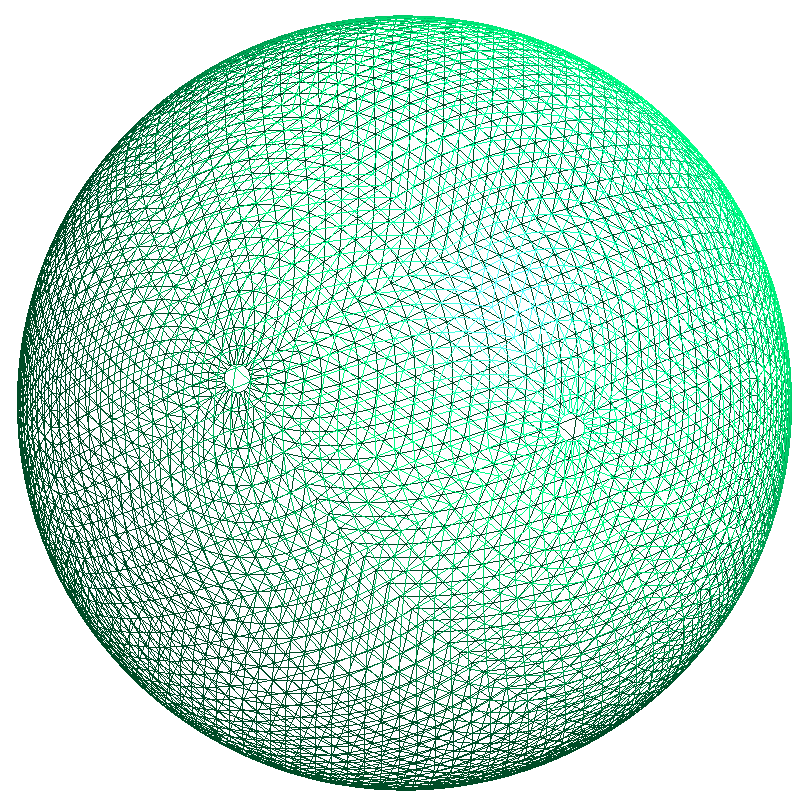
\includegraphics[width=5cm]{imgs/O32-3D.png}}\qquad\qquad\qquad
\subfloat{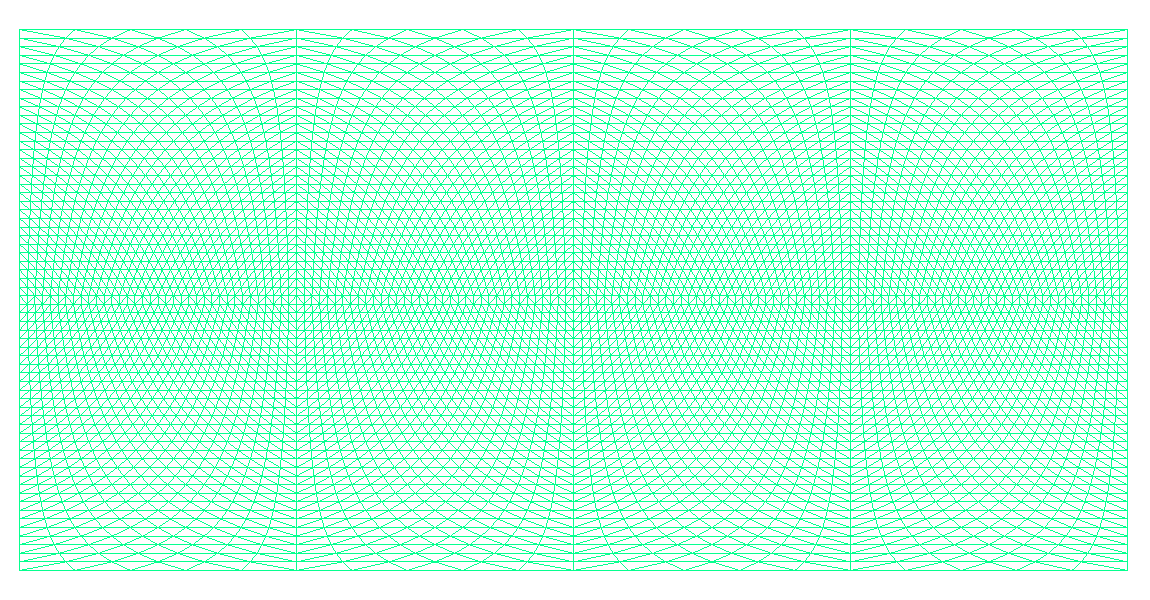
\includegraphics[width=5cm]{imgs/O32-2D.png}}
\caption{Meshes visualised in Gmsh}%
\label{fig:meshes}%
\end{figure}
%
You can now play with the command-line argument to generate 
different types of global structured meshes using the keys 
introduced in \chap{chap:global-grids}!




\section{Fortran version}
The \lista{code-meshes-C} shows how to construct a mesh 
starting from a grid.
%
\lstinputlisting[caption=Generating a mesh starting from a grid 
in \Atlas using Fortran, style=FStyle, label=code-meshes-F]{meshes-Structured.F90}
%
We first create 
a global structured grid object (see line 13). For more 
details on how to create a grid see \chap{chap:global-grids}.

We successively create the mesh object on line 15 and 16.
In particular, we first define a \inltc{atlas\_meshgenerator\_Structured} 
object that is then used to effectively generate the mesh object 
\inltc{mesh} that is an \inltc{atlas\_mesh} type.

In this simple example we took the freedom to add just one line 
line to visualize the mesh in Gmsh. In particular, on line 17 
we call \inltc{atlas\_write\_gmsh} to write a Gmsh file called 
\inlsh{mesh.msh}. Note that at the end of the program we also 
need to destroy the local object created in this program (see 
lines 19 to 21).

It is now possible to run this simple program by using 
a command-line arguments representing the keyword that 
identifies an \Atlas predefined grid. For instance, 
we can execute the following command line
%
\begin{lstlisting}[style=BashStyle]
./atlas_c-meshes-Structured
\end{lstlisting}
% 
This will produce an octahedral reduced Gaussian mesh 
(stored in mesh.msh) with 32 latitudes on one emisphere 
(i.e. 64 latitudes in total).
If we visualize it in Gmsh, we will obtain something similar
to \fig{fig:meshes-f}.
%
\begin{figure}%
\centering
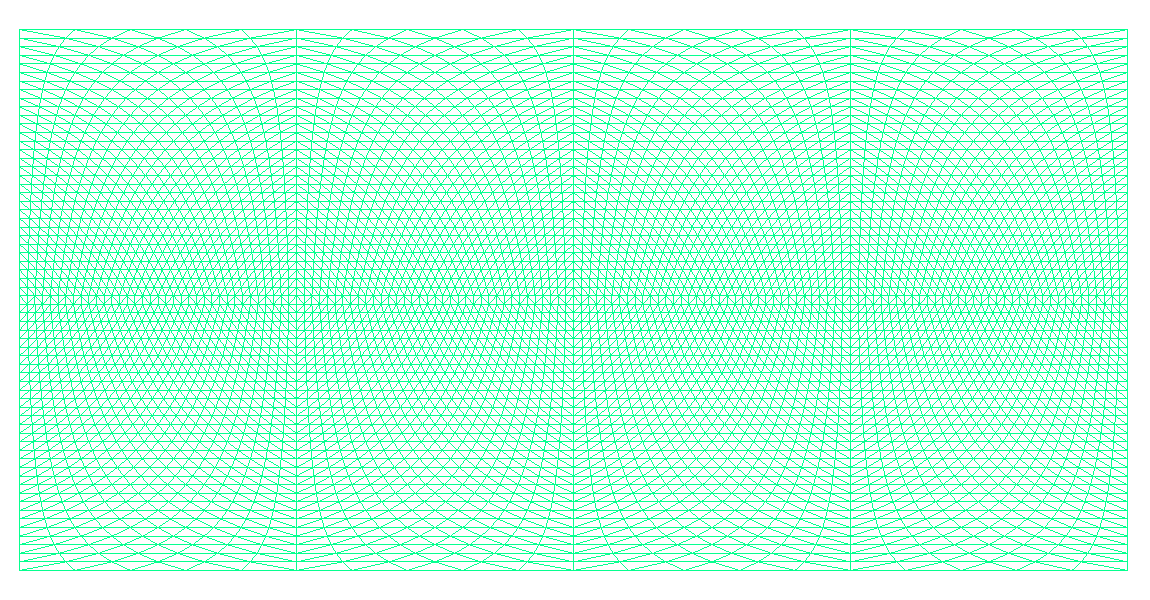
\includegraphics[width=0.5\textwidth]{imgs/O32-2D.png}
\caption{Mesh visualised in Gmsh}%
\label{fig:meshes-f}%
\end{figure}
%
You can now play with the command-line argument to generate 
different types of meshes for global grids using the keys 
introduced in \chap{chap:global-grids}!
